\todofilebegin{040\_evaluation\_validation.tex}
%%%%%%%%%%%%%%%%%%%%%%%%%%%%%%%%%%%%%%%%%%%%%%%%%%%%%%%%%%%%%%%%%%%%%%%%%%%%%%
%%%%%%%%%%%%%%%%%%%%%%%%%%%%%%%%%%%%%%%%%%%%%%%%%%%%%%%%%%%%%%%%%%%%%%%%%%%%%%
%%%%%%%%%%%%%%%%%%%%%%%%%%%%%%%%%%%%%%%%%%%%%%%%%%%%%%%%%%%%%%%%%%%%%%%%%%%%%%

\section{Evaluation and Validation}

%%%%%
%%%%%

%%%%%
%SOSflow as a tool is \textit{production capable} for the purpose of
%validating the SOS workflow performance model.
%
%As we demonstrate, even the current un-optimized code is able to scale
%out to reasonable allocation sizes and handle relatively impressive
%varieties, quantities, and rates of data flow.
%

%%%%%

%-----------------------------------------------------------------------------



%
%  I need to go through here and update all of this to
%  reflect work done at LLNL and in preparation for the
%  Scalable Tools '16 talk.
%     -Chad
%




\subsection{Testing Platform and SOS Configurations}
%%%%%
%All results were obtained by either probing (figure~\ref{probe_json})
%the daemon or by running queries against the SOSflow databases, such
%as the one in figure~\ref{example_query}.
%%%%%

%%%%%
%%%%%

%%%%%
%%%%%

%%%%%
Single node tests of SOSflow used an 8-way Xeon workstation with
Ubuntu linux, gcc, and OpenMPI.
%
Runs were performed by launching the sosd(listener) daemon along with
an sosd(db) instance as background MPI tasks.
%
The demo\_app tool was then also launched as an MPI task with varying
parameters to explore the capabilities of the sosd daemons.
%%%%%

%%%%%
%%%%%

%%%%%

%-----------------------------------------------------------------------------

\subsection{Latency}

%%%%%
When messages are received over the socket by the sosd(listener)
daemon, they are placed in an asynchronous task queue rather than
being handled immediately.
%
This allows the socket reading loop to immediately return to listening
for another connection.
%
There are three threads running inside the daemon that resolve
messages: local\_sync, node\_sync, and db\_sync.
%
The local\_sync thread picks up the incoming messages from the queue
first, unpacks the message and updates the in-memory data
structures.
%
The local\_sync message handler concludes by creating appropriate
tasks in the db\_sync queue to schedule new values for storage, and
then places the original message in the node\_sync queue for
transmission to a sosd(db) aggregator.
%%%%%

%%%%%
The latency figures shown here reveal how long a value is floating in
the asynchronous queues of the daemon before being stored in the
database.
%
Practically speaking this indicates how long it takes after a value is
published before it is available for searching by an analytics module.
%
The in situ latency graphs (figures~\ref{aciss_lat_3_situ} and
\ref{aciss_lat_24_situ}) will be discussed in more detail in the
Scalability section below.
%
Latency in the context of these graphs is \textit{not} the time cost
of calling SOSflow functions: Blocking API calls that message a daemon
over the socket are nearly constant time regardless of daemon load,
also discussed under Scalability.
%%%%%

%%%%%
When a value is inserted into the database the time\_recv field is set,
the time\_pack and time\_sent fields having already been filled by the
original source of the value.
%
Latency is calculated by subtracting the time\_sent from the
time\_recv figures.
%
When a message is migrated from a sosd(listener) instance to a
sosd(db) aggregate daemon, it is packed up together with many other
messages and sent over MPI.
%
On receipt by an sosd(db) role, those composite messages are broken
apart and immediately serviced, causing the db\_sync queue to grow
rapidly in brief bursts as large quantities of data can be arriving
all at once.
%
It is expected that the upper bound on latency for sosd(db) roles will
be higher than the in situ databases.
%%%%%

%%%%%

%-----------------------------------------------------------------------------

\subsection{Scalability}

%%%%%

%%%%%
The data store used by SOS at this time is Sqlite3.
%
It was chosen for its simplicity and essential functionality, and
because its license is open.
%
The configuration for these experiments has Sqlite3 creating a file
and writing to it, rather than representing the database only in RAM
-- though /dev/shm memory-mapped folders are used as the working
directory for the data store wherever possible.
%
For reasonable rates of data injection, Sqlite3 serves the project
well, but at larger scales it is expected that it will be replaced
with a more robust data store.
%
When the rate of value injection into SOSflow exceeds the rate at
which it is able to spool the data into the database, the queues will
fill up to the point where the only option is to discard data or
crash.
%
For the ancitipated use cases that SOSflow is targeting, this should
not be the case, but for stress tests and synthetic demos it is
certainly possible to trigger.
%%%%%

%%%%%
Precursors to this failure case can be seen in the difference between
figures~\ref{aciss_lat_3_situ} and \ref{aciss_lat_24_situ}.
%
In both cases there were 10 processes, each sending 10,000 values to
the sosd(listener) before pausing.
%
In \ref{aciss_lat_3_situ} the 10 processes pause for 0.1 seconds, and
in \ref{aciss_lat_24_situ} they pause for 0.3 seconds.
%
The slightly longer pause completely changes the shape of the latency
graph, and dramatically cuts down on the upper bound for the time a
value stayed in the asynchronous queues of the in situ daemon,
bringing it from 1.8 seconds down to 0.25 seconds.
%
The queues were able to fully drain with the 0.3 seconds pause,
whereas the 0.1 second delay gives rise to the ascending sawtooth
pattern more typical of sosd(db) ranks dealing with bundles of
messages coming in from MPI.
%%%%%

%%%%%
In the case of the in situ communication, the sawtooth shape is purely
a function of publishing in data faster than it can be written out to
the database store.
%
In the aggregate case the sawtooth is a product of data having been
generated and timestamped simultaneously across the cluster, then
being secondarily injected in an aggregate database in a
linear-per-node order of MPI message arrival.
%
The aggregator does not open all pending messages to interleave
individual values, though there will likely be refactoring to provide
more fair sharing of latency across finer grained units.
%%%%%

%%%%%
To avoid excessive queue depth and resource consumption, it is
important to ensure natural pauses exist after periods of dense value
injection so that daemon queues can flush.
%
Future work on SOSflow will add mechanisms to automatically throttle
value intake when this behavior is detected in order to increase the
robustness of the daemons.
%%%%%



%-----------------------------------------------------------------------------

\subsection{Overhead and Perturbation}

%%%%%
Synthetic stress test experiments do not give the best picture of the
overhead and perturbation of real-world applications.
%
In more realistic examples SOSflow's presence and activity in situ
resulted in just over 1\% percent increase in the execution time of
the standard LULESH simulation on NERSC's Cori supercomputer for
scales of 8 to 512 client processes.
%
See figure~\ref{cori_results} for more information about the Cori
results.
%
SOSflow processed more than 48 million data points at the largest
scale in real time, making them available for online query in the
aggregate data store with a mean queue latency time of 17.127 seconds
and a maximum of 104.42 seconds.
%%%%%

%%%%%
\begin{figure*}[!t]
\centering
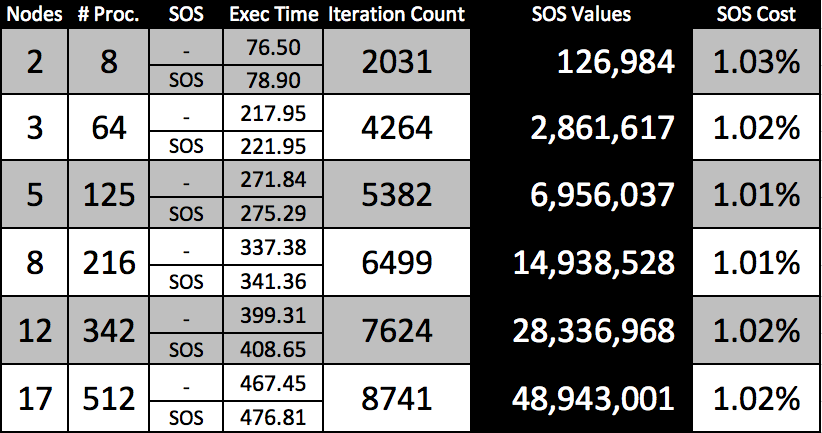
\includegraphics[width=5in]{images/cori_results.png}
\caption{Impact of SOSflow on LULESH Experiments}
\label{cori_results}
\end{figure*}
%%%%%

%\todofileend{040\_evaluation\_validation.tex}
